\chapter{Making Sound Audible}

There are two ways to make a computer-generated signal audible. It can either be sent directly to the sound card, often called the digital-to-analog-converter (DAC), or be recorded and stored to a file, for later playback. The following sections will examine these two possibilities and their implementation in C++.

\section{Recording Sound}

To record and store a sound for later playback, it must be written to a file. For digital audio recordings, there are a set of well-known and widely supported file formats with different benefits and detriments. Some are lossless, some lossy. Some are compressed, some uncompressed. Examples include MPEG-3 with its .mp3 file extension, Vorbis (.ogg), the Audio Interchange File Format (.aiff) or the Wave Audio File Format (.wav), usually referred to as WAVE. The latter is arguably the easiest to work with, as it requires relatively little configuration and stores raw, uncompressed sample data, making it very simple to write a sample buffer to a WAVE file. Consequently, the Wave Audio File Format will be further discussed.

\subsection{WAVE files}

\noindent WAVE files are part of the family of Resource Interchange File Format (RIFF) specifications, developed by Microsoft. (Wilson, 2003)

\begin{blockquote}
  \emph{The RIFF specification defines the file as a set of nested 'chunks' of data. Each chunk begins with an 8-byte chunk header. The chunk header identifies the chunk type with a 4-character ID followed by the chunk size as a 4-byte binary value.} \citebs{33}
\end{blockquote}

\noindent The first of these chunks is the top-level RIFF chunk, which contains basic information about the type of the RIFF file, e.g. that the WAVE specification is used. Then follow two sub-chunks, the Format Chunk and the Data Chunk. The first is for information concerning the file and file data's format, such as the sample rate, the number of bytes used per sample or the number of channels. The second stores the sample data and its overall size. Figure \ref{fig:wave} displays the structure of a WAVE file.

\begin{figure}[p!]
  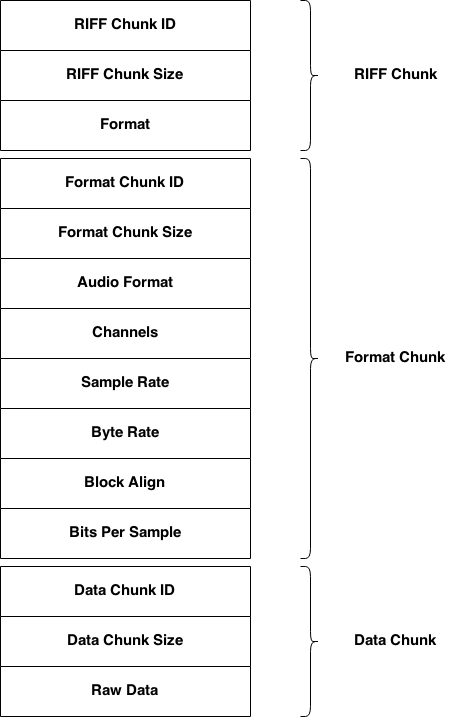
\includegraphics[scale=0.7]{img/wave}
  \caption{The WAVE file format specification.}
  \label{fig:wave}
\end{figure}

\pagebreak

\subsubsection{Discussion of WAVE file chunks}

The following list dicusses the individual chunks of a WAVE file in detail.

\begin{description}

  \item[RIFF Chunk] \hfill

  \begin{description}

    \item[RIFF Chunk ID] \hfill \\ Identifier for the family of RIFF specifications, stored as a 4-byte string (\texttt{"RIFF"}).

    \item[RIFF Chunk Size] \hfill \\ The size of everything to follow in the RIFF file. Determined after the sample data has been written to the file at the very end.

    \item[Format] \hfill \\ The specific RIFF format used, in this case the WAVE audio format. Stored as a 4-byte string (\texttt{"WAVE"}).

  \end{description}

  \item[Format Chunk] \hfill

  \begin{description}

    \item[Format Chunk ID] \hfill \\ The identifier of the sub-chunk, stored as a 4-byte string (\texttt{"fmt"}).

    \item[Format Chunk Size] \hfill \\ The size of the sub-chunk. For WAVE files, the size of the Format Chunk is always 16 (bytes).

    \item[Audio Format] \hfill \\ The type of quantization to be used for the audio data. The standard is Pulse-Code-Modulation (PCM), also called linear quantization. Setting the Audio Format to 1 means that the file uses PCM.

    \item[Channels] \hfill \\ The number of channels for the audio data. Usually either one ("mono") or two ("stereo").

    \item[Sample Rate] \hfill \\ The sample rate used for the audio data. Common values are 48000 or 44100.

    \item[Byte Rate] \hfill \\ The number of bytes to stream per second, equal to the Sample Rate times the Block Align value.

    \item[Block Align] \hfill \\ The number of bytes used per sample block, equal to the Bits Per Sample times the number of channels, divided by 8 to convert bits to bytes.

    \item[Bits Per Sample] \hfill \\ The amount of bits used to represent a single sample value. Usually samples are stored as 16-bit signed integers, so this value can be set to 16.

  \end{description}

  \item[Data Chunk] \hfill

  \begin{description}

    \item[Data Chunk ID] \hfill \\ 4-byte identifier for the Data sub-chunk (\texttt{"data"}).

    \item[Data Chunk Size] \hfill \\ The size of the sample data in bytes.

    \item[Raw Data] \hfill \\ The raw, binary sample data.

  \end{description}

\end{description}

\subsubsection{Implementation}

The \texttt{Wavefile} class implements a means to store sample data to a WAVE file. All the various chunks are stored in a simple \texttt{struct} and pre-initialized if possible. Samples can be written to an internal buffer and when the user wishes to write the recorded samples to a file, the relevant data members of the WAVE header are updated and written to disk together with the raw sample data. Listings \ref{code:wavehpp} and \ref{code:wavecpp} shows the full definition and implementation of the \texttt{Wavefile} class.

\section{Direct Output}

The second method of making sound audible is to send it to the sound card or digital-to-analog-converter (DAC). To do so, one has to interface with the Operating System's sound processing capabilities. The difficulty here is that each Operating System (OS) has its own sound API (Application Program Interface). Moreover, there may be different APIs for a single OS, as shown in Table \ref{tb:dac}. The pragmatic, cross-platform-oriented programmer does not interface with each of these APIs him- or herself, but makes use of one of the many well-documented and well-implemented Open-Source libraries, such as the RtAudio\footnote{Found at: \url{http://www.music.mcgill.ca/~gary/rtaudio/index.html}} library. This library eases the implementation of direct sound output in a digital synthesizer by adjusting to one of the many sound APIs, as needed. All the programmer needs to do is implement a simple call-back function, which the RtAudio library calls whenever the OS and the sound API request new audio data.

\begin{table}[h!]

  \begin{tabular}{c|c|c|c|}
    \cline{2-4}
    & Windows & OS X & Linux \\
    \hline
    \multicolumn{1}{|c|}{ALSA} & No & No & Yes \\
    \hline
    \multicolumn{1}{|c|}{OSS} & No & No & Yes \\
    \hline
    \multicolumn{1}{|c|}{PulseAudio} & No & No & Yes \\
    \hline
    \multicolumn{1}{|c|}{Jack} & No & Yes & Yes \\
    \hline
    \multicolumn{1}{|c|}{CoreAudio} & No & Yes & No \\
    \hline
    \multicolumn{1}{|c|}{DirectSound} & Yes & No & No \\
    \hline
    \multicolumn{1}{|c|}{ASIO} & Yes & No & No \\
    \hline
    \multicolumn{1}{|c|}{WASAPI} & Yes & No & No \\
    \hline
  \end{tabular}

  \caption{Sound APIs and what Operating Systems they are available for.}

  \label{tb:dac}

\end{table}
